\documentclass[12pt]{report}
\usepackage[utf8]{inputenc}
\usepackage{hyperref}
\usepackage[affil-it]{authblk}
\usepackage{graphicx}

\title{Réseaux intelligents et réseaux industriels}
\author{M. LIEDJI WENKACK D.%
  \thanks{Electronic address: \texttt{liedjiwenkack@gmail.com}; Corresponding author}}
\affil{University of Dschang, Cameroon\\ Master professionnel\\ Niveau: 2\\ Option : RTS}

\date{Dated: \today}

\makeatletter
\def\@maketitle{%
  \newpage
  \null
  \vskip 2em%
  \begin{center}%
  \let \footnote \thanks
    {\Large\bfseries \@title \par}%
    \vskip 1.5em%
    {\normalsize
      \lineskip .5em%
      \begin{tabular}[t]{c}%
        \@author
      \end{tabular}\par}%
    \vskip 1em%
    {\normalsize \@date}%
  \end{center}%
  \par
  \vskip 1.5em}
\makeatother


\begin{document}

\maketitle
\tableofcontents
\hypertarget{que-sont-les-ruxe9seaux-intelligents}{%
      \chapter{\texorpdfstring{C'est quoi un réseaux intelligent ?
        }{C'est quoi réseaux intelligent ?}}\label{que-sont-les-ruxe9seaux-intelligents}}

Prenons un exemple simple. Votre téléphone. Avant qu'il ne soit connecté
à l'Internet, il ne pouvait jouer que les chansons que vous aviez mises dedans. Il ne pouvait
appeler que les personnes dont vous aviez le numéro de téléphone.

\emph{Puis quelque chose de magique s'est produit. Nous l'avons connecté
      à l'internet}

Maintenant, il peut jouer n'importe quelle chanson. Vous n'êtes pas
limité à un simple numéro de contact pour vous connecter à quelqu'un.
Vous avez accès à des informations que vous tenez en main et qui ne
tiennent pas dans des To de stockage de données. C'est la puissance réseau Internet.

Internet et les smartphones, les ordinateurs sont des outils vraiment
puissants, mais le smartphone n'arrosera pas vos plantes, il n'ouvrira
pas votre porte, ou encore il ne lancera pas un processeur industriel. Ces appareils ont des capacités physiques très limitées.

Le réseau intelligent consiste à étendre la puissance des réseaux (Internet, wifi, LAN, etc...)
au-delà des ordinateurs et des smartphones à toute une série d'autres
choses, processus et environnements.

\hypertarget{comment-faire-comment-uxe9tendre-le-pouvoir-uxe0-linternet}{%
      \section{\texorpdfstring{Comment faire ? Comment étendre le pouvoir des réseaux ?
        }{Comment faire ? Comment étendre le pouvoir des réseaux ? }}\label{comment-faire-comment-uxe9tendre-le-pouvoir-uxe0-linternet}}

En plaçant autour de vous des éléments qui interagissent et ressentent
le monde physique et en les connectant au réseau afin de le rendre intelligent. Ces composants sont
des combinaisons de capteurs et d'actionneurs.

\hypertarget{quest-ce-que-le-capteur}{%
      \section{\texorpdfstring{Qu'est-ce que le capteur ?
        }{Qu'est-ce que le capteur ? }}\label{quest-ce-que-le-capteur}}

En termes simples, le capteur mesure une propriété physique. Tout comme
le capteur de température mesure la température.

\hypertarget{quest-ce-quun-actionneur}{%
      \section{\texorpdfstring{Qu'est-ce qu'un actionneur ?
        }{Qu'est-ce qu'un actionneur ? }}\label{quest-ce-quun-actionneur}}

On peut comprendre les actionneurs comme l'opposé du capteur. Comme les
capteurs convertissent les changements externes en signaux, les
actionneurs convertissent les signaux en action. Comme l'ouverture
d'une serrure de porte.

Bien sûr, avec ces capteurs et actionneurs, il faudrait du matériel
supplémentaire pour les contrôler et, si nécessaire, pour transférer les
informations sur le réseau.

\hypertarget{reseaux intelligent-changer-le-monde}{%
      \section{\texorpdfstring{Les reseaux intelligent Changent le monde
        }{Les reseaux intelligent Changent le monde }}\label{reseaux intelligent-changer-le-monde}}

Un reseaux intelligent vous permet de surveiller et d'agir sur les appareils connectés
plus étroitement que jamais. Qu'il s'agisse des industries qui gèrent
leurs machines, des agriculteurs qui contrôlent leurs cultures, des
gouvernements qui gèrent les frontières, des administrations qui
surveillent la qualité de l'air ou de l'eau, rien ne doit être contrôlé
manuellement une ou deux fois par semaine. \emph{Tout se passe en temps réel !}

Pensez aux réfrigérateurs intelligents qui vous rappellent quand vous
êtes à court de lait, ou aux plantes intelligentes qui vous rappellent
de les arroser quand elles sont à sec, les possibilités ne sont limitées
qu'à votre imagination. Nous constatons déjà de tels changements avec
les reseaux intelligents :

\begin{itemize}
      \item
            Automobiles
      \item
            Sécurité industrielle et domestique intelligente
      \item
            Domotique
      \item
            Suiveurs de fitness, montres intelligentes et articles vestimentaires
      \item
            Une agriculture autonome et efficace
\end{itemize}

\hypertarget{larchitecture-dun-projet-reseaux intelligent}{%
      \chapter{\texorpdfstring{L'architecture d'un reseau intelligent
        }{L'architecture d'un reseau intelligent }}\label{larchitecture-dun-projet-reseaux intelligent}}

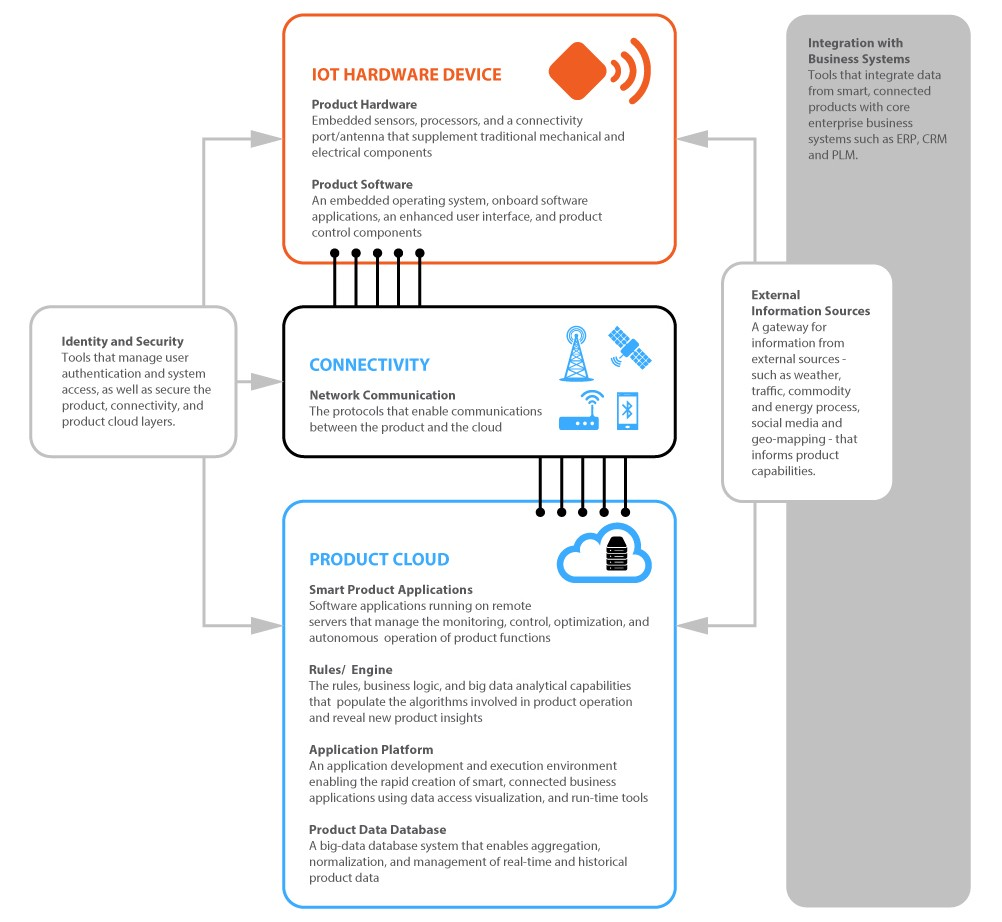
\includegraphics[width=5.83333in,height=3.88889in]{figs/iot_arch.jpeg}

L'architecture d'un projet reseaux intelligent comporte trois grands volets

\begin{itemize}
      \item
            Composant hardware : le dispositif physique qui interagit avec
            l'environnement
      \item
            Connectivité : le lien entre votre appareil et le cloud
      \item
            produits du cloud  : serveurs qui prennent des données, les traitent,
            les stockent dans des bases de données, donnent des commandes,
            effectuent des analyses, servent les données de manière utile à tous
            les différents acteurs. Vous connaissez peut-être la connectivité et
            le cloud, car ils sont identiques à ceux de tout site web et de toute
            application. Mais ici, vous devrez également gérer le matériel de
            l'appareil, ce qui apporte des complexités supplémentaires.
\end{itemize}

\hypertarget{dispositif-matuxe9riel-de-lreseaux intelligent}{%
      \section{\texorpdfstring{Dispositif matériel des reseaux intelligents
        }{Dispositif matériel des réseaux intelligents }}\label{dispositif-matuxe9riel-de-lreseaux intelligent}}

C'est la partie la plus complexe et la plus unique d'un produit reseaux intelligent.
Vous voudriez créer un dispositif spécifique à vos besoins.

Pour un système d'irrigation intelligent, vous devrez ajouter des
capteurs qui détectent le niveau d'humidité et interagissent avec la
pompe, mais pour un système de sécurité domestique, vous aurez besoin de
capteurs pour détecter les mouvements ou de caméras et traiter cela pour
les intrus et ensuite alerter avec une alarme ou des notifications.

Il faut sélectionner ou construire sur mesure des composants matériels
pour répondre à un cas d'utilisation spécifique et des logiciels qui
fonctionneront sur ce matériel.

\hypertarget{produit-matuxe9riel}{%
      \section{\texorpdfstring{Produit Matériel
        }{Produit Matériel }}\label{produit-matuxe9riel}}

Le matériel sera doté d'un \textbf{processeur/contrôleur central} qui sera
responsable de l'exécution de la logique et de capteurs et d'actionneurs
qui collecteront les données et agiront sur les commandes.

Considérez ce processeur/contrôleur central comme le cerveau qui est
responsable de toute la logique et la peau, les yeux, les mains, les
jambes comme des capteurs et des actionneurs qui détectent et rapportent
au cerveau et le cerveau donne l'ordre d'effectuer ensuite une action
sur la base de cela.

Sur la base de cette unité centrale, il existe des cartes permettant de concevoir un réseau intelligent et basées sur
des microcontrôleurs et des cartes à microprocesseur.

\hypertarget{basuxe9-sur-des-microcontruxf4leurs}{%
      \section{\texorpdfstring{Basé sur des microcontrôleurs :
        }{Basé sur des microcontrôleurs : }}\label{basuxe9-sur-des-microcontruxf4leurs}}

\begin{itemize}
      \item
            Arduino Uno, Mega : facile à développer et beaucoup de broches pour
            connecter les périphériques, idéal pour le prototypage
      \item
            Cartes ESP8266 / ESP32 : dispose d'une connectivité WiFi et Bluetooth,
            d'un faible coût (ESP8266 coûte environ 3 \$), de nombreuses
            ressources à développer.
      \item
            Les cartes de la série STM32F : complexes à développer, faciles à
            produire et à fabriquer, les plus utilisées en production.
\end{itemize}

\hypertarget{basuxe9-sur-un-microprocesseur}{%
      \section{\texorpdfstring{Basé sur un microprocesseur :
        }{Basé sur un microprocesseur : }}\label{basuxe9-sur-un-microprocesseur}}

\begin{itemize}
      \item
            Raspberry Pi : communauté géniale, facile à développer, peut faire
            fonctionner des systèmes d'exploitation comme Linux, Windows
      \item
            Beagle bone : carte open source, peut faire fonctionner les systèmes d'exploitation android, ubuntu et autres
            Linux, possède un stockage flash intégré
\end{itemize}

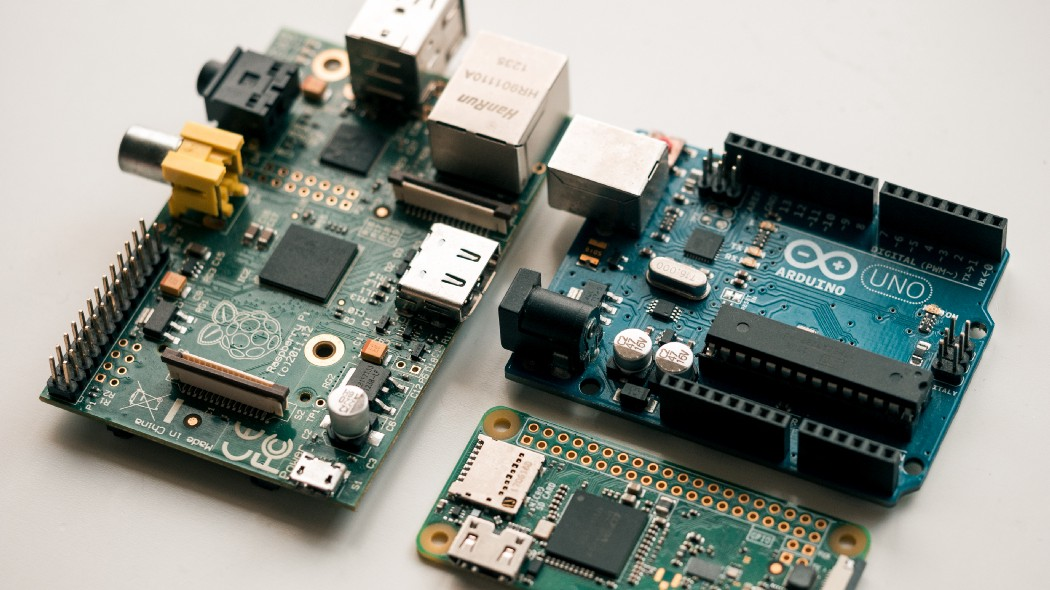
\includegraphics[width=4.16667in,height=2.77778in]{figs/hardware_devices.jpg}

framboise pi modèle b, framboise pi zéro, et Arduino Uno

Sur ces cartes, vous remarquerez un microcontrôleur et des microprocesseurs (la grosse puce noire au milieu).
Il y a aussi beaucoup de broches marquées de chiffres. Ces broches sont des
broches d'E/S qui sont utilisées pour se connecter à tous les capteurs ou
actionneurs que vous souhaitez utiliser. Il est également possible d'utiliser plusieurs
microcontrôleurs/microprocesseurs, car vous pouvez établir une
communication entre eux.

Il suffit donc de choisir une carte qui correspond à vos besoins et,
grâce à ces broches IO, vous pouvez utiliser tous les capteurs que vous
voulez. Tout capteur que vous choisissez sera très probablement
compatible avec toutes les cartes.

Voici quelques exemples de capteurs et d'actionneurs :

\begin{itemize}
      \item
            Capteurs de température et d'humidité
      \item
            Capteur de pression
      \item
            Capteur de proximité
      \item
            Capteur de gaz
      \item
            Capteur de fumée
      \item
            Capteur d'alcool
      \item
            Capteur à ultrasons
      \item
            Relais : fermeture et ouverture électroniques des circuits
            (interrupteurs) moteurs
\end{itemize}

Disons que vous voulez construire un système de lutte contre l'incendie,
vous pouvez choisir n'importe quelle carte (Arduino, ESP8266, etc...),
connecter des capteurs de fumée et un interrupteur de relais pour le
sprinkler. Chaque fois que le capteur de fumée détecte de la fumée,
donnez l'ordre au relais de déclencher l'arrosage. Bien sûr, vous devez
écrire cette logique quelque part. C'est là que le logiciel du produit
entre en jeu.

\hypertarget{produits-logiciels-et-protocoles-de-communication}{%
      \chapter{\texorpdfstring{Produits logiciels et protocoles de
              communication
        }{Produits logiciels et protocoles de communication }}\label{produits-logiciels-et-protocoles-de-communication}}

Comme le code doit être compilé spécifiquement pour le microcontrôleur
ou le microprocesseur et en raison de l'absence d'un système
d'exploitation comme Linux, Windows qui fait abstraction des variations
matérielles, les logiciels et les outils qui seront utilisés pour le
développement dépendent largement de la puce que vous sélectionnez. Bien
qu'il existe de nombreux cadres qui tentent de prendre en charge un
grand nombre de puces.

Les choses que vous devez vérifier :

\begin{itemize}
      \item
            Arduino Framework : supporte une variété de cartes et de puces comme
            toutes les puces Arduino, ESP8266, ESP32, STM32
      \item
            FreeRTOS : système d'exploitation très populaire pour les
            microcontrôleurs, léger, supporte une variété de puces
      \item
            Amazon FreeRTOS : la version d'Amazon du RTOS gratuit qui se connecte
            de manière transparente au cloud AWS IoT et prend en charge de
            nombreuses autres fonctionnalités comme les mises à jour Over the air,
            le provisionnement
      \item
            Apache Mynewt : axé sur le développement de produits reseaux intelligent sans fil
\end{itemize}

Le fabricant de la puce que vous sélectionnez peut également disposer
d'outils de développement, comme la STM, qui propose ses propres outils
de développement pour ses puces. N'oubliez pas de vérifier cela aussi.

Si vous utilisez une carte reseaux intelligent plus puissante comme le pi framboise qui
peut faire fonctionner des systèmes d'exploitation à part entière comme
Linux, Windows, alors bien sûr, cela se résume à développer une
application Linux ou Windows. Mais il vous faudra quand même faire
quelques interactions matérielles pour obtenir des données des capteurs.

Le choix de la technologie pour la connectivité dépend de
l'environnement dans lequel vous allez mettre le produit. Par exemple,
la plupart des reseaux intelligent domestiques utiliseront le WiFi, car il est
facilement accessible dans chaque maison, mais si vous construisez un
compteur de qualité de l'air dans la ville, le WiFi pourrait ne pas être
disponible dans cette ville, vous pourriez décider d'utiliser le
GSM/GPRS.

Maintenant, pour l'agriculture, vous avez des centaines de capteurs
répartis sur des hectares, vous voudriez utiliser une communication
radio avec un centre de contrôle central et ensuite transmettre toutes
ces données à l'internet si nécessaire. Les technologies de
communication sont donc choisies en fonction des cas d'utilisation.
Certaines technologies de communication sont :

\begin{itemize}
      \item
            WiFi : convient aux installations intérieures telles que les appareils
            IoT à la maison et au bureau
      \item
            RFID/NFC : le cas d'utilisation le plus courant est le contrôle
            d'accès par carte
      \item
            GSM/GPRS : pour les appareils autonomes d'extérieur
      \item
            Bluetooth : choix le plus courant pour les articles portables et les
            appareils qui peuvent être contrôlés à l'aide d'un smartphone,
            également utilisé pour le provisionnement wifi ( configuration des
            identifiants wifi d'un appareil), peut également créer un maillage
            Bluetooth pour plusieurs appareils.
      \item
            LoRaWAN : idéal pour les produits d'infrastructure industrielle et
            publique pour une communication d'une portée de 3 à 5 km, conçu pour
            les dispositifs d'un réseau intelligent, peut créer un réseau avec des passerelles sur une
            grande surface
      \item
            NB-IoT : Le réseau intelligent à bande étroite est une technologie de communication
            cellulaire spécialement conçue pour alimenter la communication d'un réseau intelligent, à
            très faible puissance.
\end{itemize}

La prochaine étape consiste à mettre en place des \textbf{protocoles de
      communication} qui seront utilisés pour la communication entre votre
appareil et le cloud.

\hypertarget{protocoles-de-communication-par-messagerie}{%
      \section{\texorpdfstring{Protocoles de communication par messagerie
        }{Protocoles de communication par messagerie }}\label{protocoles-de-communication-par-messagerie}}

\begin{itemize}
      \item
            HTTP : le plus facile à prendre en charge, avec beaucoup de surcharge,
            non synchrone, idéal pour les demandes uniques, pas pour une
            communication continue
      \item
            WebSockets HTTP : basés sur HTTP donc beaucoup de surcharge, mais
            supportent une communication continue
      \item
            MQTT : protocole de réseau intelligent le plus couramment utilisé (la plupart des
            solutions comme Amazon FreeRTOS l'utilisent par défaut), basé sur le
            modèle de publication/abonnement, très léger, pas d'encombrement
            inutile, très souple
      \item
            AMQP : open-source, orientation des messages, file d'attente, routage,
            support point à point et modèle de publication-abonnement
\end{itemize}

\hypertarget{cloud-de-produits}{%
      \chapter{\texorpdfstring{produits du cloud: Serveur central
        }{produits du cloud : Serveur central }}\label{cloud-de-produits}}

Le cloud est l'endroit où résident tous les traitements, analyses et
bases de données. Lorsque le cloud reçoit les données brutes de milliers
d'appareils, il doit transformer les données, appliquer une logique
commerciale, stocker les données d'une manière qui soit utile pour les
récupérer et alimenter les applications du produit IoT. Il doit
également maintenir l'état, la santé de tous les appareils de terrain.
Poussez les mises à jour aériennes pour tout changement nécessaire et
gardez une trace des appareils qui sont mis à jour et de ceux qui
restent.

Le cloud est également responsable de l'interaction entre les
applications (applications et sites web) et le dispositif. Si des tâches
ou des commandes sont données par l'application, le cloud est
responsable de l'envoi de ces commandes/tâches aux appareils et doit
également suivre si la commande est exécutée avec succès.

Pour concevoir l'architecture en cloud, il convient d'envisager les
éléments suivants

\begin{itemize}
      \item
            Séparer la couche de réception des messages de la couche de traitement
            pour éviter tout étranglement des messages
      \item
            Pensez toujours aux appareils qui se déconnectent et fonctionnent mal
      \item
            Prévoir des mises à jour en direct (il y aura toujours des bogues et
            des changements dans les exigences)
      \item
            Toutes les communications doivent être sécurisées
      \item
            Mettre en place un système d'authentification afin qu'un appareil ne
            puisse pas publier de messages pour un autre appareil et ne puisse pas
            s'abonner à des chaînes qui ne lui sont pas autorisées
      \item
            Maintenir l'état actuel de chaque appareil dans le cloud
      \item
            Comme la taille des données va bientôt devenir énorme, choisissez une
            base de données qui s'adapte bien
\end{itemize}

Il existe de nombreuses solutions de cloud computing que l'on peut
utiliser :

\begin{itemize}
      \item
            Suite Microsoft Azure IoT
      \item
            Plate-forme reseaux intelligent de Google Cloud
      \item
            Plate-forme AWS IoT : bien intégrée avec Amazon FreeRTOS
      \item
            Plate-forme Watson IoT
\end{itemize}

L'utilisation d'un cloud serait très bénéfique car elle éviterait de
nombreuses erreurs de conception et permettrait de construire en gardant
à l'esprit les meilleures pratiques.

Vous serez bombardé de choix en matière de matériel, de capteurs, de
logiciels et de communication. Vous avez la possibilité de choisir
exactement ce que vous voulez et seulement ce dont vous avez besoin.
C'est peut-être un peu écrasant au début, mais c'est vraiment amusant.

\hypertarget{suxe9curituxe9-des-ruxe9seaux-intelligents}{%
      \chapter{\texorpdfstring{Sécurité des réseaux intelligents
        }{Sécurité des réseaux intelligents }}\label{suxe9curituxe9-des-ruxe9seaux-intelligents}}

\hypertarget{quels-sont-certains-des-risques-encourus-par-une-organisation}{%
      \section{\texorpdfstring{Quels sont certains des risques encourus par
              une organisation ?
        }{Quels sont certains des risques encourus par une organisation ? }}\label{quels-sont-certains-des-risques-encourus-par-une-organisation}}

Les dispositifs reseaux intelligent actuels ont un faible degré de contrôle de la
sécurité informatique et de faibles capacités de cryptage, ce qui les
rend vulnérables aux menaces potentielles. Les acteurs de la menace
peuvent tirer parti des vulnérabilités des dispositifs, comme dans les
exemples suivants :

\begin{itemize}
      \item
            La compromission des systèmes de contrôle environnemental et des
            appareils intelligents (par exemple, cafetière, chauffage et
            électricité) dans les espaces de travail physiques pourrait entraîner
            des pertes de bénéfices (par exemple, altération des contrôles de
            température dans une salle de serveurs, entraînant un
            dysfonctionnement des équipements)
      \item
            Obtenir un accès non autorisé aux contrôles de sécurité des bâtiments
            de l'entreprise (par exemple, déverrouillage des portes, visionnement
            des caméras de surveillance)
      \item
            Prendre le contrôle des appareils multifonctions pour perturber
            malicieusement l'accès à Internet (par exemple, l'attaque du réseau de
            zombies Mirai
      \item
            Accès à des microphones à distance sur les appareils reseaux intelligent pour écouter
            des conversations sensibles
      \item
            Prendre le contrôle des caractéristiques d'une voiture (par exemple,
            altération des freins d'un véhicule)
      \item
            Contrôle de l'équipement médical d'un hôpital (par exemple,
            interférence avec les systèmes d'imagerie par résonance magnétique
            {[}IRM{]})
      \item
            l'accès à des données sensibles ou à des informations personnelles
            (par exemple, les noms des clients et les cartes de crédit) par
            l'intermédiaire de dispositifs reseaux intelligent non sécurisés qui sont connectés
            aux réseaux des entreprises
\end{itemize}

\hypertarget{comment-puis-je-suxe9curiser-les-dispositifs-reseaux intelligent}{%
      \section{\texorpdfstring{Comment puis-je sécuriser les dispositifs reseaux intelligent ?
        }{Comment puis-je sécuriser les dispositifs reseaux intelligent ? }}\label{comment-puis-je-suxe9curiser-les-dispositifs-reseaux intelligent}}

Avant d'introduire des dispositifs reseaux intelligent dans votre organisation, vous
devez rechercher les protocoles de sécurité et comprendre les types de
données que les dispositifs envoient et reçoivent. À mesure que de plus
en plus de produits reseaux intelligent sont introduits sur le lieu de travail, votre
organisation a besoin de plans et de politiques pour minimiser la
possibilité d'incidents de cybersécurité sur votre réseau. Vos plans et
politiques doivent tenir compte des considérations suivantes :

\begin{itemize}
      \item
            Restreindre les dispositifs reseaux intelligent personnels pour se connecter à un
            réseau distinct (par exemple, le Wi-Fi invité
      \item
            Modification des mots de passe par défaut sur les appareils reseaux intelligent. Si
            les règles relatives aux mots de passe le permettent, utilisez des
            phrases de passe, plutôt que des mots de passe, sur tous les appareils
            reseaux intelligent sur le lieu de travail
      \item
            Utiliser l'authentification à deux facteurs pour les dispositifs ou
            les applications afin d'ajouter une couche de sécurité supplémentaire
      \item
            S'assurer que les données générées par les éléments de l'reseaux intelligent sont
            cryptées
      \item
            Désactivation de toute fonctionnalité de connexion automatique (par
            exemple, plug and play)
      \item
            Appliquer des correctifs de sécurité et des mises à jour aux
            dispositifs reseaux intelligent (si le produit le permet)
      \item
            Surveiller, détecter et corriger tout problème de sécurité de l'reseaux intelligent
      \item
            Recherche d'études et de cotes de sécurité sur les fabricants et les
            produits
\end{itemize}

\hypertarget{les-meilleures-pratiques-de-suxe9curituxe9-de-lreseaux intelligent}{%
      \section{\texorpdfstring{Les bonnes pratiques de sécurité des réseaux intelligents
        }{Les bonnes pratiques de sécurité des réseaux intelligents}}\label{les-meilleures-pratiques-de-suxe9curituxe9-de-lreseaux intelligent}}

\emph{L'un des plus grands défis des reseaux intelligents est le
      casse-tête de sécurité qui l'accompagne. Ce problème est exacerbé dans
      les entreprises, où les appareils connectés contrôlent souvent de
      grosses machines dangereuses, ou envoient et reçoivent des données
      sensibles. Si les reseaux intelligent peut apporter de nouvelles données et des
      informations utiles, il introduit également de nouvelles vulnérabilités
      dans votre entreprise. Il est donc essentiel que les entreprises
      prennent en compte les implications d'un déploiement des reseaux intelligent en matière
      de sécurité avant d'aller de l'avant.}

La sécurisation d'une infrastructure reseaux intelligent nécessite une stratégie de
sécurité rigoureuse et approfondie. Cette stratégie exige que vous
sécurisiez les données dans le cloud, que vous protégiez l'intégrité des
données lors de leur transit sur l'internet ou  le reseaux local et que vous mettiez
en place des dispositifs de sécurité. Chaque couche renforce l'assurance
de sécurité de l'infrastructure globale. Selon l'article de l'IEEE sur
la sécurité des reseaux intelligent, les bonnes pratiques pour les entreprises, les
écoles, les usines et les autres organisations qui cherchent à améliorer
leur sécurité de reseaux intelligent sont:

\hypertarget{rendre-le-matuxe9riel-inviolable}{%
      \section{\texorpdfstring{\textbf{Rendre le matériel inviolable}
        }{Rendre le matériel inviolable }}\label{rendre-le-matuxe9riel-inviolable}}

Certains dispositifs reseaux intelligent peuvent fonctionner en permanence sans
surveillance et ne pas être soumis à la sécurité qu'implique cette
observation humaine directe et fréquente. Bien qu'il soit préférable de
maintenir les dispositifs relativement isolés afin que seules quelques
personnes désignées y aient accès physiquement, en particulier dans le
cas de dispositifs totalement inattendus, il peut être avantageux de les
rendre inviolables ou inviolables. Cette forme de durcissement des
terminaux peut contribuer à empêcher les intrus potentiels d'accéder aux
données. Elle peut également permettre de se défendre contre un pirate
informatique qui achète puis arme des dispositifs. La sécurité physique
des terminaux peut inclure, par exemple, de petits dispositifs en
plastique simples, des verrous de port et des caches de caméra, qui
verrouillent les ports USB et Ethernet et couvrent les ouvertures des
webcams. Le verrouillage des ports permet d'empêcher l'entrée de
logiciels malveillants indésirables. Certaines méthodes de protection
contre les manipulations désactivent le dispositif lorsqu'il est
manipulé. En tant que meilleure pratique, le durcissement des terminaux
sécurisés implique probablement une approche par couches qui exige des
attaquants qu'ils contournent divers obstacles conçus pour protéger le
dispositif et ses données contre l'accès et l'utilisation illicites.


Au niveau du matériel/logiciel de démarrage, des mots de passe forts au
niveau du démarrage ou l'obligation de démarrer le périphérique à partir
du stockage local seulement peuvent constituer des approches
judicieuses. Les vulnérabilités connues doivent être protégées, telles
que les ports TCP/UDP ouverts, les ports série ouverts, les invites de
mot de passe ouvertes, les endroits où injecter du code comme les
serveurs web, les communications non cryptées et les connexions radio.
Pour l'expédition, un emballage inviolable permettra au propriétaire du
dispositif de savoir si un dispositif a été ouvert avant son arrivée. Le
nombre et la force de la sécurité à chaque niveau dépendent du modèle de
menace, des niveaux de risque acceptables et de la commodité souhaitée.

\hypertarget{pruxe9voir-des-mises-uxe0-jourrappels-de-microprogrammes}{%
      \section{\texorpdfstring{Prévoir des mises à jour/rappels de
              microprogrammes
        }{Prévoir des mises à jour/rappels de microprogrammes }}\label{pruxe9voir-des-mises-uxe0-jourrappels-de-microprogrammes}}

Inévitablement, les vulnérabilités seront découvertes après le
déploiement des dispositifs. Les dispositifs doivent pouvoir être
réparés ou mis à niveau. Naturellement, les microprogrammes des
appareils ne doivent être modifiables qu'avec la signature numérique
appropriée. Dans l'état actuel des choses, les vendeurs et les
fabricants d'appareils ont une petite incitation financière à assurer la
mise à jour continue des correctifs de l'reseaux intelligent, puisque les revenus
proviennent de la vente de l'appareil et non de sa maintenance.
L'entretien des appareils reseaux intelligent peut réduire les revenus.

En outre, les vendeurs ne sont pas légalement tenus responsables de la maintenance
continue des appareils au-delà des ventes initiales et la concurrence
pousse les vendeurs à faire des économies, ce qui nuit à la qualité, à
l'efficacité et à la rapidité de mise sur le marché. Bien que ces
facteurs n'aient peut-être pas été critiques avant l'reseaux intelligent, la nature
interconnectée des dispositifs reseaux intelligent place la barre à un niveau supérieur
en termes de fonctionnalité et de responsabilité. La tendance des
vendeurs à planifier l'obsolescence des appareils afin de maximiser les
profits par la poursuite des ventes plutôt que par l'entretien des
appareils existants est également préjudiciable.

En outre, les dispositifs reseaux intelligent ne sont pas conçus ou configurés efficacement pour
répondre aux mises à jour OTA (over the air), ce qui entraîne, au mieux,
des procédures coûteuses et, au pire, ingérables. Dans l'état actuel des
choses, de nombreux dispositifs reseaux intelligent sont inutilisables et, de ce fait,
ne peuvent être sécurisés. Les chercheurs ont observé que l'omniprésence
de l'reseaux intelligent et le placement de dispositifs reseaux intelligent non sécurisés et non
surveillés dans les foyers et les entreprises augmentera de manière
exponentielle, ouvrant ainsi la voie aux pirates informatiques pour
exploiter les vulnérabilités critiques {[}9{]}. Outre leur obsolescence
prévue, de nombreux dispositifs reseaux intelligent ont tout simplement un cycle de vie
limité. Les entreprises doivent être légalement tenues responsables de
la surveillance et de la maintenance des dispositifs pendant les cycles
de vie prescrits et convenus. Pour cela, il faut établir des normes et
mettre en place une législation.

En outre, les fournisseurs doivent faire preuve de transparence et de franchise en ce qui concerne le cycle
de vie des dispositifs, notamment en termes de politiques de service et
d'entretien, y compris la durée pendant laquelle ils prévoient de
prendre en charge leurs dispositifs. Ils doivent jouer un rôle actif en
fournissant des détails sur les correctifs et les mises à niveau ainsi
que sur les risques de sécurité et les préoccupations en matière de vie
privée, en veillant à ce que le consommateur et/ou l'utilisateur soit
informé des changements de politique, de fonctionnalité et de sécurité.
Le cycle de vie complet du dispositif reseaux intelligent doit être pris en compte, en
commençant par la fabrication où les références de sécurité doivent être
"générées, allouées et fournies dans les dispositifs de manière
sécurisée" {[}8{]}. Les délibérations doivent également intégrer le
cycle de vie du fabricant d'origine. Lorsque le fournisseur d'origine
n'existe plus, il devient impossible de retrouver les références afin de
corriger les vulnérabilités et les failles de sécurité, et les
fournisseurs sont inévitablement remplacés et/ou disparaissent ou font
faillite.

\hypertarget{effectuer-des-tests-dynamiques}{%
      \section{\texorpdfstring{Effectuer des tests dynamiques
        }{Effectuer des tests dynamiques }}\label{effectuer-des-tests-dynamiques}}

Il est essentiel que les dispositifs reseaux intelligent soient soumis à des tests
approfondis et qu'ils établissent une base de référence minimale en
matière de sécurité. Les tests statiques ne sont pas destinés ou conçus
pour trouver les vulnérabilités qui existent dans les composants
disponibles sur le marché, tels que les processeurs et la mémoire dans
lesquels peut se trouver un composant de l'application globale. Les
tests dynamiques, en revanche, sont capables d'exposer à la fois les
faiblesses du code et les défauts ou vulnérabilités sous-jacents
introduits par le matériel et qui peuvent ne pas être visibles à
l'analyse statique. Les tests dynamiques peuvent découvrir des
vulnérabilités qui sont créées lorsqu'un nouveau code est utilisé sur
d'anciens processeurs. Nous recommandons aux fabricants qui achètent du
matériel et des logiciels à des tiers de procéder à des tests dynamiques
pour s'assurer que les éléments sont sécurisés.

\hypertarget{pruxe9ciser-les-procuxe9dures-de-protection-des-donnuxe9es-relatives-uxe0-luxe9limination-des-dispositifs}{%
      \section{\texorpdfstring{Préciser les procédures de protection des
              données relatives à l'élimination des dispositifs
        }{Préciser les procédures de protection des données relatives à l'élimination des dispositifs }}\label{pruxe9ciser-les-procuxe9dures-de-protection-des-donnuxe9es-relatives-uxe0-luxe9limination-des-dispositifs}}

Les appareils finissent par devenir obsolètes et les utilisateurs
peuvent décider de les jeter. Les appareils doivent être mis au rebut
sans exposer les données privées. Il s'agit d'une question de sécurité,
car les appareils mis au rebut de manière inappropriée peuvent être
convertis à des fins malveillantes. Il s'agit d'une question de vie
privée car, s'il est laissé en service ou s'il est mis au rebut de
manière inappropriée, le matériel obsolète pourrait être utilisé pour
révéler des informations personnelles sur l'utilisateur ou d'autres
acteurs de l'écosystème de l'reseaux intelligent. Il en va de même pour les dispositifs
reseaux intelligent qui sont vendus à des seconds propriétaires ou qui deviennent des
équipements standard dans les maisons et sont transportés lors de la
vente de la maison. Nous suggérons aux fabricants de préparer un plan
officiel pour que les utilisateurs puissent assainir et se débarrasser
des dispositifs reseaux intelligent obsolètes. Les pratiques de l'industrie dans
d'autres domaines prescrivent une politique de "mise au rebut, recyclage
ou destruction" (DRD) avec une révision périodique du plan afin de
déterminer quels dispositifs doivent être éliminés et comment s'en
débarrasser. Certains fabricants encouragent les utilisateurs à se
débarrasser de leurs produits directement par l'intermédiaire du
fabricant. Cela peut être judicieux pour les ordinateurs portables et
les serveurs, mais pour les appareils reseaux intelligent qui peuvent être petits et bon
marché, ou qui font partie d'un appareil beaucoup plus grand (comme un
réfrigérateur), des aménagements spéciaux peuvent être nécessaires. Les
utilisateurs individuels, lors de l'achat d'un produit reseaux intelligent d'occasion,
peuvent tenter d'identifier les informations d'identification
personnelle (IIP) ou les informations d'authentification telles que le
nom d'utilisateur et le mot de passe (UNPW) qui restent stockées sur le
dispositif, ou qui sont accessibles par le dispositif, ou qui doivent
être stockées ailleurs afin d'utiliser le dispositif. Par exemple,
l'Amazon Echo Dot exige des utilisateurs qu'ils stockent les mots de
passe de leur routeur de réseau Wi-Fi sur un serveur Amazon. Il faut se
demander si les utilisateurs doivent ou non déterminer une politique
individuelle de DRD, ce qui peut inclure la suppression d'informations
de tout endroit accessible par Internet autre que l'appareil lui-même.
Dans l'état actuel des choses, les utilisateurs sont mal préparés, ne
possèdent pas les compétences numériques nécessaires pour naviguer dans
ce type de sécurité, et sont mal équipés pour comprendre les complexités
du stockage des mots de passe dans les appareils connectés. L'exposition
à ces complexités vient souvent trop tard, comme ce fut le cas lors de
la récente révélation que les photocopieurs et les télécopieurs modernes
ont des disques durs qui conservent des copies de documents. Même les
utilisateurs d'entreprises dont le service informatique a été formé à la
sécurité n'étaient pas conscients de ce fait. Les implications pour la
sécurité dans l'exemple ci-dessus sont nombreuses et montrent à quel
point il est facile de ne pas tenir compte de failles de sécurité
majeures.

\hypertarget{utiliser-lauthentification-forte}{%
      \section{\texorpdfstring{Utiliser l'authentification forte
        }{Utiliser l'authentification forte }}\label{utiliser-lauthentification-forte}}

Les dispositifs reseaux intelligent ne doivent pas utiliser des identifiants faciles à
deviner, tels que le nom d'utilisateur ou le mot de passe de
l'administrateur. Les appareils ne doivent pas utiliser d'identifiants
par défaut qui sont invariables sur plusieurs appareils et ne doivent
pas inclure de portes dérobées ni de paramètres de mode de débogage
(identifiants secrets établis par le programmeur de l'appareil) car une
fois devinés, ils peuvent être utilisés pour pirater de nombreux
appareils. Chaque appareil devrait avoir un nom d'utilisateur/mot de
passe unique par défaut, éventuellement imprimé sur son boîtier, et de
préférence réinitialisable par l'utilisateur. Les mots de passe doivent
être suffisamment sophistiqués pour résister aux devinettes et aux
méthodes dites de force brute. Dans la mesure du possible, nous
recommandons une authentification à deux facteurs (2FA), qui exige que
l'utilisateur utilise à la fois un mot de passe et une autre forme
d'authentification qui ne repose pas sur la connaissance de
l'utilisateur, comme un code aléatoire généré par SMS. Pour les
applications reseaux intelligent, nous encourageons tout particulièrement l'utilisation
de l'authentification contextuelle (CAA), également connue sous le nom
d'authentification adaptative, dans laquelle l'utilisation
d'informations contextuelles et d'algorithmes d'apprentissage machine
évalue en permanence le risque de malveillance sans déranger
l'utilisateur en exigeant une authentification. Si le risque est élevé,
l'abonné (ou le hacker) se verra demander un jeton multi-facteur pour
continuer à avoir accès.

\hypertarget{utiliser-un-cryptage-fort-et-des-protocoles-suxe9curisuxe9s}{%
      \section{\texorpdfstring{Utiliser un cryptage fort et des protocoles
              sécurisés
        }{Utiliser un cryptage fort et des protocoles sécurisés }}\label{utiliser-un-cryptage-fort-et-des-protocoles-suxe9curisuxe9s}}

Même si les mots de passe des appareils sont sécurisés, les
communications entre les appareils peuvent être piratées. Dans l'reseaux intelligent, il
existe de nombreux protocoles, notamment Bluetooth, Zigbee, Z-Wave,
6LoWPAN, Thread, Wi-Fi, cellulaire, NFC, Sigfox, Neul et LoRaWAN. Selon
le protocole et les ressources informatiques disponibles, un appareil
peut être plus ou moins capable d'utiliser un cryptage fort. Les
fabricants doivent examiner leur situation au cas par cas et utiliser le
cryptage le plus fort possible, de préférence IPsec et/ou TLS/SSL. Il
peut y avoir des cas où le cryptage n'est pas souhaitable, comme dans
les messages de sécurité de base (BSM) SAE J2735, que les voitures de
communication sans fil peuvent utiliser pour éviter les collisions. Dans
ces cas, les messages peuvent être envoyés en clair et vérifiés à l'aide
de signatures numériques. Toutefois, il convient de prendre en
considération les implications de l'omission du cryptage. Dans le cas de
la norme SAE J2735, les BSM pourraient être utilisés pour alerter
faussement les systèmes de gestion des collisions et immobiliser une
automobile. Il n'y a pas de réponse toute faite qui évite de devoir
réfléchir soigneusement aux modèles de menace prévus et aux
vulnérabilités qui seront tolérées. Si les données sont transmises non
cryptées et non signées, des précautions doivent être prises pour
s'assurer que les fausses données ont peu ou pas de chance de causer des
dommages.

\hypertarget{ruxe9duire-la-largeur-de-bande-des-appareils}{%
      \section{\texorpdfstring{Réduire la largeur de bande des appareils
        }{Réduire la largeur de bande des appareils }}\label{ruxe9duire-la-largeur-de-bande-des-appareils}}

Récemment, des attaques DDoS ont été menées à grande échelle par des
armées de dispositifs reseaux intelligent mal protégés qui sont devenus des systèmes
zombies dans le cadre de campagnes mondiales massives. La plupart des
dispositifs reseaux intelligent sont constitués de composants de base dont les capacités
réseau sont largement surchargées pour la fonction qu'ils sont censés
remplir, ce qui provoque un encombrement des réseaux domestiques et
contribue potentiellement à des coûts énormes pour les cibles des
attaques DDoS par reseaux intelligent.

Si, à l'avenir, 50 milliards d'appareils étaient connectés à l'internet, et si nous supposons (sur la base des conditions
actuelles) que 1,1 \% d'entre eux sont compromis et sous contrôle à
distance coordonné, cela représente 55 millions d'appareils IoT
malveillants. Supposons que chaque dispositif soit capable de générer un
trafic d'attaque à débit de ligne équivalent au Gigabit Ethernet (81
274-1 488 096 images par seconde), par exemple, le système sur puce
(SoC) ARM9 intègre deux connexions de ce type, et il coûte moins de 5
dollars par puce. En utilisant cette armée de zombies de 55 millions
d'appareils pour générer des événements DDoS, les attaquants pourraient
générer entre 4,47 et 81,8 billions d'images par seconde ou 55 petabits
par seconde. Cela dépasse de loin les capacités défensives d'un seul
fournisseur de services. Une attaque de cette ampleur dépasserait
l'interface réseau la plus rapide construite à ce jour (300 Gbps) par
une marge de 183 333 à 1. Il n'y a pas de bon moyen de réduire le trafic
malveillant produit par ces systèmes, si ce n'est en l'étouffant à la
source. Nous recommandons aux fabricants d'appareils de limiter la
quantité de trafic réseau que les appareils reseaux intelligent peuvent générer aux
niveaux raisonnablement nécessaires pour remplir leurs fonctions.

Il est très peu nécessaire qu'un réfrigérateur connecté à Internet puisse
diffuser des messages ICMP (Internet Control and Management Protocol) à
des vitesses de l'ordre du gigabit par seconde. Bien que certains
réfrigérateurs soient équipés d'écrans vidéo, il est fort probable
qu'ils n'aient pas besoin de capacités de téléchargement à grande
vitesse. Les vendeurs doivent utiliser des limitations de bande passante
au niveau du matériel et du noyau pour limiter les taux de transmission
du réseau à des niveaux raisonnables pour les tâches de chaque appareil.
De telles limitations rendent beaucoup plus difficile l'utilisation d'un
appareil par un attaquant dans une attaque DDoS, même s'il l'a
complètement compromis.

En outre, les appareils doivent être programmés pour s'autosurveiller des comportements inhabituels et se remettre aux
paramètres d'usine lorsqu'un comportement alarmant est détecté. S'il
n'est pas possible de réinitialiser les appareils aux paramètres
d'usine, ils doivent au moins redémarrer pour effacer le code que
l'attaquant a en mémoire. Maintenant, supposons que les 55 millions de
dispositifs IoT malveillants mentionnés ci-dessus aient une bande
passante atténuée renforcée par le matériel/le noyau, disons 10 trames
Ethernet par seconde, alors leur profil d'attaque potentiel global tombe
à 550 millions de trames par seconde, et pas plus de 6,6 térabits par
seconde.

C'est près de 150 000 fois moins, et bien qu'elle soit encore
trop importante pour un seul défenseur, une attaque de cette taille peut
être stoppée par un ensemble de défenseurs répartis. Des contrôles
supplémentaires au niveau du noyau dans les dispositifs qui remarquent
et atténuent de grandes quantités de trafic téléchargé ou arrêtent
d'autres comportements inattendus pourraient réduire davantage les
capacités destructrices des dispositifs compromis sans nécessiter
d'efforts héroïques de la part des défenseurs du réseau. Nous
recommandons donc d'examiner sérieusement les exigences de performance
de chaque dispositif et de mettre en place des limitations modestes
difficiles à contourner. Cela augmentera considérablement la sécurité
des dispositifs reseaux intelligent et permettra de mettre en œuvre en toute sécurité un
nombre beaucoup plus important de ces dispositifs à l'avenir.

\hypertarget{diviser-les-ruxe9seaux-en-segments}{%
      \section{\texorpdfstring{Diviser les réseaux en segments
        }{Diviser les réseaux en segments }}\label{diviser-les-ruxe9seaux-en-segments}}

Séparez le réseau en réseaux locaux plus petits en utilisant des VLAN,
des plages d'adresses IP ou une combinaison de ceux-ci. Les
segmentations de réseau sont utilisées dans les politiques de sécurité
de pare-feu de nouvelle génération pour identifier clairement une ou
plusieurs interfaces source et destination sur la plate-forme. Chaque
interface du pare-feu doit être affectée à une zone de sécurité avant de
pouvoir traiter le trafic. Cela permet aux organisations de créer des
zones de sécurité pour représenter les différents segments connectés au
pare-feu et contrôlés par celui-ci. Par exemple, les administrateurs de
la sécurité peuvent attribuer tous les dépôts de données des titulaires
de cartes ou des patients dans un segment de réseau identifié par une
zone de sécurité (par exemple, les données des clients).

L'administrateur peut ensuite élaborer des politiques de sécurité qui
n'autorisent que certains utilisateurs, groupes d'utilisateurs,
applications spécifiques ou autres zones de sécurité à accéder à la zone
des données des clients - empêchant ainsi tout accès interne ou externe
non autorisé aux données stockées dans ce segment. Ce type de solution
est plus courant dans les applications industrielles mais peut être
utile dans des circonstances plus larges. Un réseau privé séparé et
détaché pour un système de sécurité, peut-être avec un canal dédié à une
"base d'origine" dans le cas d'un système de sécurité domestique,
pourrait suffire. Si le système doit utiliser l'internet, un réseau
privé virtuel (VPN) peut être mis en place.

\chapter{Conception et mise en oeuvre d'un réseau intélligent}

\section*{Plan à suivre:}
\begin{itemize}
      \item{Presentation de raspberry pi}
      \item{Rappel de programmation python}
      \item{Utilisation des différentes couches de l'architecture d'un réseau intélligent}
      \item{Utilisation d'un protocole de réseau intelligent}
      \item{Réalisation d'un réseau intélligent sécurisé.}
\end{itemize}

\end{document}
